% This file was created with tikzplotlib v0.9.17.
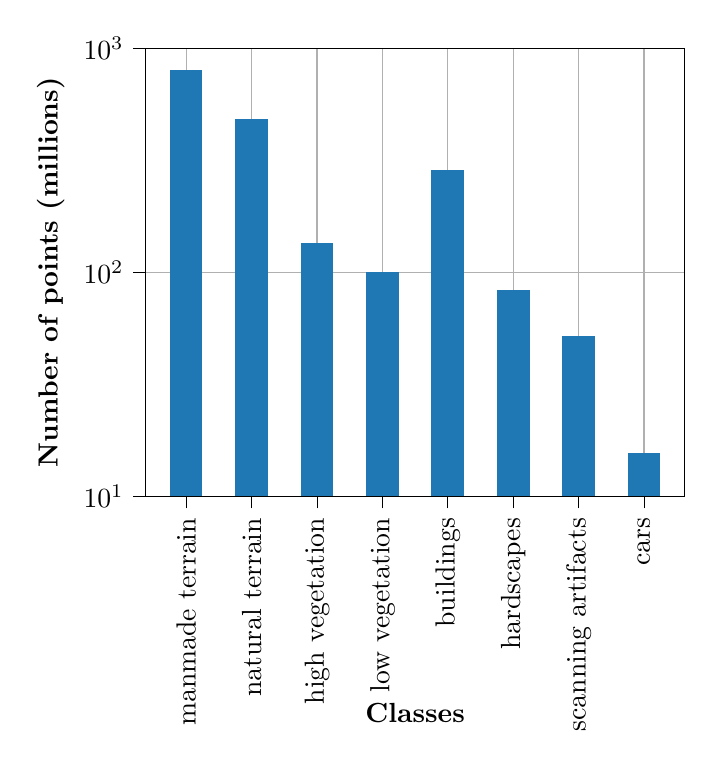
\begin{tikzpicture}

\definecolor{color0}{rgb}{0.12156862745098,0.466666666666667,0.705882352941177}

\begin{axis}[
log basis y={10},
tick align=outside,
tick pos=left,
x grid style={white!69.0196078431373!black},
every axis x label/.style={at={(current axis.south)},below=25mm},
xlabel={\textbf{Classes}},
xmajorgrids,
xmin=-0.625, xmax=7.625,
xtick style={color=black},
xtick={0,1,2,3,4,5,6,7},
xticklabel style={rotate=90.0},
xticklabels={
  manmade terrain,
  natural terrain,
  high vegetation,
  low vegetation,
  buildings,
  hardscapes,
  scanning artifacts,
  cars
},
y grid style={white!69.0196078431373!black},
ylabel={\textbf{Number of points (millions)}},
ymajorgrids,
ymin=10, ymax=1000,
ytick={10, 100, 1000},
ymode=log,
ytick style={color=black}
]
\draw[draw=none,fill=color0] (axis cs:-0.25,0) rectangle (axis cs:0.25,796.491236);
\draw[draw=none,fill=color0] (axis cs:0.75,0) rectangle (axis cs:1.25,480.979226);
\draw[draw=none,fill=color0] (axis cs:1.75,0) rectangle (axis cs:2.25,135.634808);
\draw[draw=none,fill=color0] (axis cs:2.75,0) rectangle (axis cs:3.25,99.971504);
\draw[draw=none,fill=color0] (axis cs:3.75,0) rectangle (axis cs:4.25,285.746985);
\draw[draw=none,fill=color0] (axis cs:4.75,0) rectangle (axis cs:5.25,83.466775);
\draw[draw=none,fill=color0] (axis cs:5.75,0) rectangle (axis cs:6.25,51.979923);
\draw[draw=none,fill=color0] (axis cs:6.75,0) rectangle (axis cs:7.25,15.609275);
\end{axis}

\end{tikzpicture}
